% !TEX root = ../notes_unsupervisedlearning.tex
% Chapter 14: World Models and Vision-Language-Action Models
%%%%%%%%%%%%%%%%%%%%%%%%%%%%%%%%%%%%%%%%%%%%%%%%%%%%%%%%%%%%%%%%%%%%%%

\chapter{World Models and Vision-Language-Action Models}\index{World Models}\index{VLA}\index{Embodied AI}
\newthought{Simulate, imagine, then act in the real world.}

%═══════════════════════════════════════════════════════════════════════
% BLOCK 1: INTRODUCTION
%═══════════════════════════════════════════════════════════════════════

\section{The Why}

\marginnote{Humans imagine consequences before acting---can machines learn to do the same?}

Model-free RL learns from experience, but:
\begin{itemize}
    \item \textbf{Sample inefficient}: Millions of environment interactions
    \item \textbf{Unsafe}: Learning by trial-and-error can be dangerous
    \item \textbf{No transfer}: Must relearn for each new task
\end{itemize}

\textbf{Model-based RL} learns a model of the world, enabling:
\begin{itemize}
    \item \textbf{Planning}: Simulate actions before taking them
    \item \textbf{Imagination}: Generate synthetic experience for training
    \item \textbf{Sample efficiency}: Learn from fewer real interactions
\end{itemize}

\textbf{Vision-Language-Action (VLA) models} represent the frontier: systems that see, understand language, and act in the physical world.

\subsection{Hands-On Experience}

\begin{marginfigure}
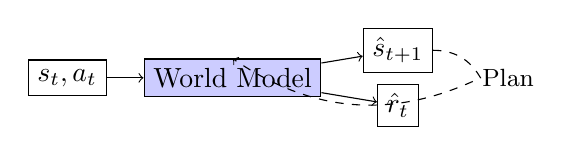
\begin{tikzpicture}[scale=0.7]
    % World model
    \node[draw, rectangle, fill=blue!20, minimum width=2cm] (wm) at (0,0) {World Model};
    % Input
    \node[draw, rectangle] (s) at (-3,0) {$s_t, a_t$};
    % Output
    \node[draw, rectangle] (sp) at (3,0.5) {$\hat{s}_{t+1}$};
    \node[draw, rectangle] (r) at (3,-0.5) {$\hat{r}_t$};

    \draw[->] (s) -- (wm);
    \draw[->] (wm) -- (sp);
    \draw[->] (wm) -- (r);

    % Planning loop
    \draw[->, dashed] (sp.east) to[bend left] (4.5,0) to[bend left] (wm.north);
    \node at (5,0) {\small Plan};
\end{tikzpicture}
\caption{World model predicts next state and reward, enabling mental simulation.}
\end{marginfigure}

Imagine you're learning to play a video game:
\begin{enumerate}
    \item After playing briefly, you can \textit{imagine} what happens if you jump
    \item You simulate different strategies in your head
    \item You execute the best plan in the real game
\end{enumerate}

This is \textbf{planning with a learned model}: act in imagination, then act in reality.

\subsection{Learning Objectives}

After this lecture, you will be able to:
\begin{enumerate}
    \item Explain model-based RL and its advantages over model-free methods
    \item Describe world model architectures (Dreamer, IRIS)
    \item Implement curiosity-driven exploration
    \item Understand VLA architectures (RT-1, RT-2, OpenVLA)
    \item Articulate the path from foundation models to embodied agents
\end{enumerate}

%═══════════════════════════════════════════════════════════════════════
% BLOCK 2: MAIN THEORY
%═══════════════════════════════════════════════════════════════════════

\section{Model-Based Reinforcement Learning}

\marginnote{Learn a model, then plan with it.}

\subsection{The Dynamics Model}

Learn $f_\theta$ to predict:
\begin{equation}
    \hat{s}_{t+1}, \hat{r}_t = f_\theta(s_t, a_t)
\end{equation}

\textbf{Training}: Supervised learning on collected transitions $(s, a, r, s')$.

\subsection{Planning with the Model}

\textbf{Model Predictive Control (MPC)}:
\begin{enumerate}
    \item At state $s$, simulate many action sequences
    \item Evaluate cumulative reward for each
    \item Execute first action of best sequence
    \item Repeat at next state
\end{enumerate}

\begin{algorithm}[H]
\caption{MPC with Learned Model}
\begin{algorithmic}[1]
\Require Current state $s$, model $f_\theta$, horizon $H$, samples $N$
\For{$i = 1$ to $N$}
    \State Sample action sequence $a_1^i, \ldots, a_H^i$
    \State $\hat{s} \gets s$
    \State $R_i \gets 0$
    \For{$t = 1$ to $H$}
        \State $\hat{s}, \hat{r} \gets f_\theta(\hat{s}, a_t^i)$
        \State $R_i \gets R_i + \gamma^{t-1} \hat{r}$
    \EndFor
\EndFor
\State \Return $a_1^{i^*}$ where $i^* = \arg\max_i R_i$
\end{algorithmic}
\end{algorithm}

\subsection{Model Error and Compounding}

\marginnote{Model errors compound over long horizons.}

Small prediction errors accumulate:
\begin{equation}
    \text{error at step } H \approx H \cdot \epsilon_{\text{single-step}}
\end{equation}

\textbf{Mitigation}: Short planning horizons, ensemble models, re-planning frequently.


\section{World Models}

\marginnote{World models: compress observations into latent space, predict in latent space.}

\subsection{Ha \& Schmidhuber (2018)}

Architecture:
\begin{enumerate}
    \item \textbf{Vision (V)}: VAE encodes observations to latent $z$
    \item \textbf{Memory (M)}: RNN predicts future latents
    \item \textbf{Controller (C)}: Simple policy on $(z, h)$
\end{enumerate}

\begin{figure}[h]
\centering
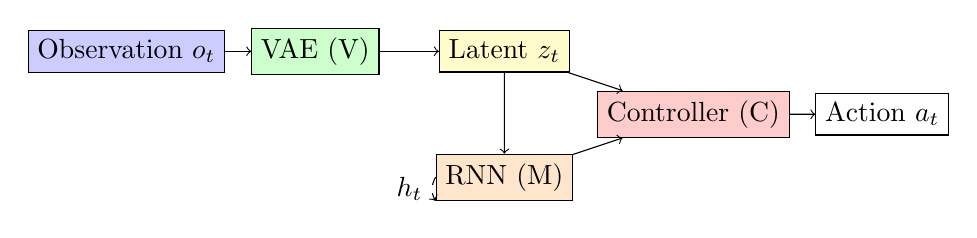
\begin{tikzpicture}[scale=0.8]
    \node[draw, rectangle, fill=blue!20] (obs) at (0,0) {Observation $o_t$};
    \node[draw, rectangle, fill=green!20] (vae) at (3,0) {VAE (V)};
    \node[draw, rectangle, fill=yellow!20] (z) at (6,0) {Latent $z_t$};
    \node[draw, rectangle, fill=orange!20] (rnn) at (6,-2) {RNN (M)};
    \node[draw, rectangle, fill=red!20] (ctrl) at (9,-1) {Controller (C)};
    \node[draw, rectangle] (act) at (12,-1) {Action $a_t$};

    \draw[->] (obs) -- (vae);
    \draw[->] (vae) -- (z);
    \draw[->] (z) -- (rnn);
    \draw[->] (z) -- (ctrl);
    \draw[->] (rnn) -- (ctrl);
    \draw[->] (ctrl) -- (act);
    \draw[->, dashed] (rnn.west) to[bend right] node[left] {$h_t$} (rnn.south west);
\end{tikzpicture}
\caption{World Models architecture: V compresses, M predicts, C acts.}
\end{figure}

\textbf{Key insight}: Train V and M on real experience, then train C entirely in imagination (dream).

\subsection{Dreamer}

\marginnote{Dreamer: state-of-the-art latent world model.}

Dreamer learns:
\begin{itemize}
    \item \textbf{Representation model}: $p(s_t | s_{t-1}, a_{t-1}, o_t)$
    \item \textbf{Transition model}: $p(s_t | s_{t-1}, a_{t-1})$
    \item \textbf{Reward model}: $p(r_t | s_t)$
    \item \textbf{Decoder}: $p(o_t | s_t)$
\end{itemize}

Actor-critic in imagination:
\begin{enumerate}
    \item Imagine trajectories using transition model
    \item Estimate values using imagined rewards
    \item Update policy to maximize imagined return
\end{enumerate}


\section{Exploration and Curiosity}

\marginnote{Sparse rewards $\to$ need intrinsic motivation to explore.}

\subsection{Intrinsic Motivation}

Add \textbf{intrinsic reward} for visiting novel states:
\begin{equation}
    r_{\text{total}} = r_{\text{extrinsic}} + \beta \cdot r_{\text{intrinsic}}
\end{equation}

\subsection{Curiosity-Driven Exploration}

\textbf{ICM} (Intrinsic Curiosity Module):
\begin{equation}
    r_{\text{intrinsic}} = \|f_\theta(s_t, a_t) - s_{t+1}\|^2
\end{equation}

High prediction error $\to$ novel state $\to$ high reward.

\textbf{Problem}: Noisy TV problem---random noise is unpredictable but not interesting.

\subsection{Random Network Distillation (RND)}

\begin{itemize}
    \item Fixed random network $f$ maps states to features
    \item Learnable network $\hat{f}$ tries to match $f$
    \item Intrinsic reward: $\|f(s) - \hat{f}(s)\|^2$
\end{itemize}

Novel states are hard to match because $\hat{f}$ hasn't seen them.


\section{Vision-Language Models for Robotics}

\marginnote{VLMs: understand images and text together.}

\subsection{From CLIP to Robotics}

Foundation models provide:
\begin{itemize}
    \item \textbf{Visual understanding}: Recognize objects, scenes, attributes
    \item \textbf{Language grounding}: Connect words to visual concepts
    \item \textbf{Common sense}: Implicit knowledge about the world
\end{itemize}

\textbf{Key question}: How to connect perception and language to action?

\subsection{PaLM-E: Embodied Multimodal Reasoning}

\begin{itemize}
    \item Inject visual tokens into large language model
    \item Model can reason about images and plan actions
    \item Output: natural language plans or action tokens
\end{itemize}


\section{Vision-Language-Action Models}

\marginnote{VLAs: the next step in embodied AI.}

\subsection{RT-1: Robotics Transformer}

\begin{itemize}
    \item Input: Image + language instruction
    \item Output: Discretized robot actions
    \item Trained on 130k real robot demonstrations
\end{itemize}

\begin{figure}[h]
\centering
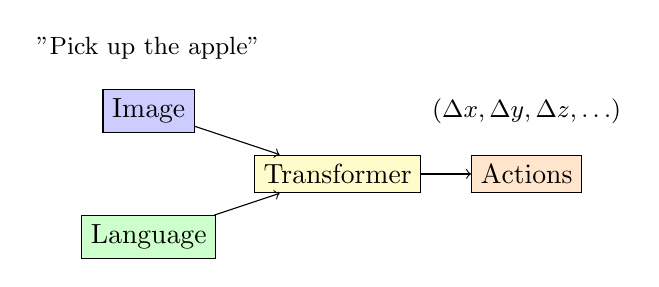
\begin{tikzpicture}[scale=0.8]
    \node[draw, rectangle, fill=blue!20] (img) at (0,1) {Image};
    \node[draw, rectangle, fill=green!20] (lang) at (0,-1) {Language};
    \node[draw, rectangle, fill=yellow!20, minimum width=2cm] (enc) at (3,0) {Transformer};
    \node[draw, rectangle, fill=orange!20] (act) at (6,0) {Actions};

    \draw[->] (img) -- (enc);
    \draw[->] (lang) -- (enc);
    \draw[->] (enc) -- (act);

    \node at (0,2) {\small "Pick up the apple"};
    \node at (6,1) {\small $(\Delta x, \Delta y, \Delta z, \ldots)$};
\end{tikzpicture}
\caption{VLA architecture: image + language $\to$ transformer $\to$ robot actions.}
\end{figure}

\subsection{RT-2: VLM as Robot Policy}

\begin{itemize}
    \item Fine-tune vision-language model (PaLI) for action prediction
    \item Actions encoded as text tokens (e.g., "move arm 0.1 forward")
    \item Inherits VLM's reasoning and generalization
\end{itemize}

\subsection{OpenVLA: Open-Source VLA}

\begin{itemize}
    \item 7B parameter model trained on Open X-Embodiment dataset
    \item Supports multiple robot embodiments
    \item Open weights for research
\end{itemize}


\section{Towards Embodied AI}

\marginnote{The ultimate test of intelligence: acting in the physical world.}

\subsection{Sim-to-Real Transfer}

Train in simulation, deploy on real robot:
\begin{itemize}
    \item \textbf{Domain randomization}: Vary simulation parameters
    \item \textbf{System identification}: Match sim to real
    \item \textbf{Real-world fine-tuning}: Adapt with real data
\end{itemize}

\subsection{Open Challenges}

\begin{itemize}
    \item \textbf{Safety}: Robots can cause harm
    \item \textbf{Generalization}: Kitchen $\neq$ warehouse $\neq$ hospital
    \item \textbf{Data}: Robot data is expensive to collect
    \item \textbf{Multimodality}: Touch, sound, proprioception
\end{itemize}


\section{Course Synthesis}

\marginnote{The full arc: from clustering to embodied agents.}

\begin{figure}[h]
\centering
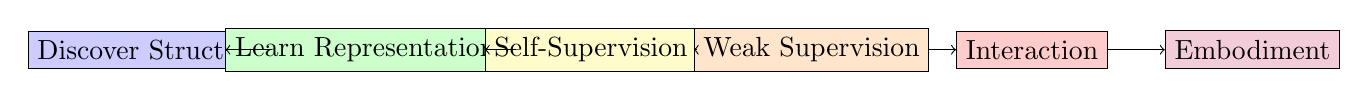
\begin{tikzpicture}[node distance=0.8cm, scale=0.7]
    \node[draw, rectangle, fill=blue!20] (struct) at (0,0) {Discover Structure};
    \node[draw, rectangle, fill=green!20, right of=struct, xshift=2cm] (repr) {Learn Representations};
    \node[draw, rectangle, fill=yellow!20, right of=repr, xshift=2cm] (self) {Self-Supervision};
    \node[draw, rectangle, fill=orange!20, right of=self, xshift=2cm] (weak) {Weak Supervision};
    \node[draw, rectangle, fill=red!20, right of=weak, xshift=2cm] (interact) {Interaction};
    \node[draw, rectangle, fill=purple!20, right of=interact, xshift=2cm] (embody) {Embodiment};

    \draw[->] (struct) -- (repr);
    \draw[->] (repr) -- (self);
    \draw[->] (self) -- (weak);
    \draw[->] (weak) -- (interact);
    \draw[->] (interact) -- (embody);
\end{tikzpicture}
\caption{The course arc: from structure to embodied intelligence.}
\end{figure}


%═══════════════════════════════════════════════════════════════════════
% BLOCK 3: STUDENT ACTIVATION
%═══════════════════════════════════════════════════════════════════════

\section{Examples \& Exercises}

\subsection{Exercise 1: World Model Design}

You want to learn a world model for a driving simulator. Design the architecture:
\begin{enumerate}
    \item What's the input?
    \item What should it predict?
    \item How would you train it?
\end{enumerate}

\textbf{Solution}:
\begin{enumerate}
    \item Input: Camera image (or latent), vehicle state, action (steering, throttle)
    \item Predict: Next image/latent, reward (distance traveled), done flag (collision)
    \item Train: Collect rollouts, supervised learning on $(s_t, a_t) \to (s_{t+1}, r_t)$
\end{enumerate}

\subsection{Exercise 2: Curiosity Trade-offs}

A robot explores a room. The TV shows random static. Why might curiosity-driven exploration spend too much time watching TV?

\textbf{Solution}: Random static is inherently unpredictable---the world model can never predict it well. Prediction error stays high, so intrinsic reward stays high. The agent keeps watching, even though it's learning nothing useful.

\subsection{Exercise 3: VLA Advantages}

Why might a VLA trained on internet data generalize better than a robot-only model?

\textbf{Solution}: Internet data contains vast knowledge about objects, physics, and common sense. A VLA inherits this: it "knows" that apples go in fruit bowls, that heavy things need more force, that "clean up" means putting things away. A robot-only model must learn this from scratch.


\section{Self-Reflection \& Recap}

\subsection{Reflection Questions}
\begin{enumerate}
    \item Why is model-based RL more sample-efficient but potentially less accurate?
    \begin{quote}
        \textit{It learns from imagined experience, but model errors compound. If the model is wrong, the policy optimizes for the wrong objective.}
    \end{quote}

    \item How do VLAs leverage pre-trained vision-language knowledge?
    \begin{quote}
        \textit{They inherit semantic understanding (what objects are), spatial reasoning (where things are), and common sense (how the world works) from web-scale pre-training.}
    \end{quote}
\end{enumerate}

\subsection{Key Concepts}
\begin{itemize}
    \item \textbf{World models} enable planning in imagination
    \item \textbf{Curiosity} drives exploration beyond sparse rewards
    \item \textbf{VLAs} unify vision, language, and action
    \item \textbf{Embodied AI} is the frontier of representation learning
    \item Foundation models are becoming robot brains
\end{itemize}

\subsection{Course Conclusion}

\newthought{We began with the question:} how do we find structure in data without labels? We explored classical clustering and dimensionality reduction, then moved to learned representations with VAEs and self-supervised learning. We saw how weak supervision, self-training, and human feedback can bootstrap learning. Finally, we arrived at reinforcement learning and embodied agents---systems that learn to perceive, reason, and act in the world.

\marginnote{The future belongs to systems that can learn from experience.}

The common thread throughout: \textbf{structure emerges from data}. Whether we discover it through clustering, learn it through reconstruction, or refine it through interaction---unsupervised and self-supervised learning form the foundation of modern AI.

\begin{figure}[h]
\centering
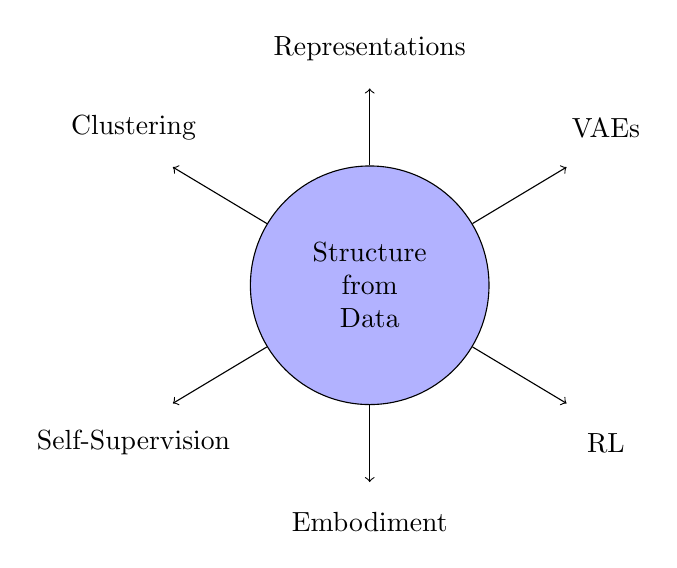
\begin{tikzpicture}
    \node[draw, circle, fill=blue!30, minimum size=3cm] (core) at (0,0) {\parbox{2.5cm}{\centering Structure\\from\\Data}};
    \node at (-3,2) {Clustering};
    \node at (3,2) {VAEs};
    \node at (-3,-2) {Self-Supervision};
    \node at (3,-2) {RL};
    \node at (0,3) {Representations};
    \node at (0,-3) {Embodiment};

    \draw[->] (core) -- (-2.5,1.5);
    \draw[->] (core) -- (2.5,1.5);
    \draw[->] (core) -- (-2.5,-1.5);
    \draw[->] (core) -- (2.5,-1.5);
    \draw[->] (core) -- (0,2.5);
    \draw[->] (core) -- (0,-2.5);
\end{tikzpicture}
\caption{The unifying theme: learning structure from data.}
\end{figure}

\textit{What comes next?} As foundation models grow more capable and robots more dexterous, the line between digital and physical AI will blur. Systems that perceive, reason, and act---grounded in the physical world, guided by language, and learning from interaction---will define the next era of artificial intelligence.
